
\section{Experiments and Results}
We address the following questions in the experiments section:

1. How much benefit is possible with different strategies of interventions in comparison with no intervention?

2. How do different strategies fare in comparison to the base strategy of performing all interventions at the first time step ($t_1 = t_2 = 1$) in non-adaptive case?
What are the effects of performing interventions at different time steps with the overall budget distributed in a skewed manner?

3. How do different strategies fare in comparison with the base strategy in adaptive case? Given a $\tau$, how long should one wait for the information before performing interventions? 

4. What is the impact of probability of infection $p$ on the interventions strategies performed at a current time step in both adaptive and non-adaptive cases?

\subsection{Dataset description and Methods}
The Dendrograms corresponding to the SIR epidemic spread are generated for the following colloboration networks: General Relativity and Quantum Cosmology collaboration network (CA-GrQC) and the High Energy Physics - Theory collaboration network (CA-HepTh). The details of these graphs are provided in Table \ref{tab:datasets}.
\begin{table}
\centering

\begin{tabular}{|c|c|c|}
\hline
    \textbf{Graph} &  \textbf{Nodes} & \textbf{Edges} \\
    \hline
    CA-GrQc & 5242 & 14496 \\
    CA-HepTh & 9877 & 14496 \\
\hline
\end{tabular}
\caption{Dataset description}
\label{tab:datasets}
\end{table}

Each dendrogram is a directed graph having multiple connected components with each component having a set of nodes sources. Each node has a timestep associated with it that corresponds to the time at which it is infected. The node either recovers or is removed in the next step before which it infects some subset of its susceptible neighbors.

In all our experiments, we assume interventions are performed at two time steps: $t_1 = 1$ and $t_2$, i.e. the first intervention is always done at time step 1. A strategy for intervention is to pick the time step for $t_2$. The budget $B$ is divided between the two interventions as follows: at most $B_1$ (resp. $B_2$) interventions allowed at $t_1$ (resp. $t_2$). We perform our LP rounding algorithm using Gurobi software to obtain the following results.

\begin{figure}[!h]
    \centering
    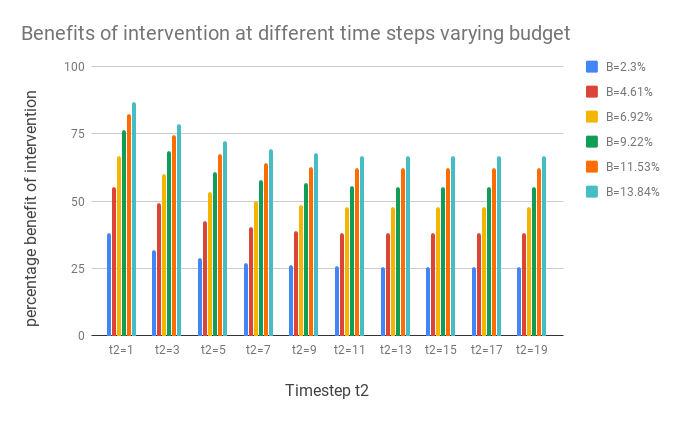
\includegraphics[height = 5cm, width = 8cm]{benefit.png}
    \caption{Benefits of interventions: GrQc}
    \label{fig:grqc_benefit}
\end{figure}

\subsection{Benefit of different intervention strategies}
We run our rounding algorithm using various strategies $t_2$ Budget values $B$ setting $B_1 = B_2 = \frac{B}{2}$. Let $a$ the average number of infections over all the dendrograms. The benefit of an intervention strategy is the percentage reduction in the average number of infections over all the dendrograms. The closer it is to 100\% the better the strategy. In Figure \ref{fig:grqc_benefit} we present the benefits of different intervention strategy on the GrQc network. As we increase the budget $B$ for a fixed strategy its benefit consistently increases. The plot shows that the strategy with lower $t_2$ value has the higher benefit for a fixed budget $B$. But all the strategies with $t_2 \geq 7$ have the same benefit with no increase for a fixed $B$. In plots we show $B$ as a percentage of the average number of infected over all the dendrograms.

\subsection{Non adaptive Interventions: Comparison of strategies w.r.t. base strategy for both budget distributions}
We call the intervention strategy with $t_1 = t_2 = 1$ as base strategy as it uses all budget $B$ at the first time step providing the optimal benefit. We consider two types of budget distributions in this experiment: (B.i) equally divided $B$ between $t_1$ and $t_2$, and (B.ii) allocate $\frac{3B}{4}$ to $t_1$ and $\frac{B}{4}$ to $t_2$. 
\begin{figure}[!h]
    \centering
    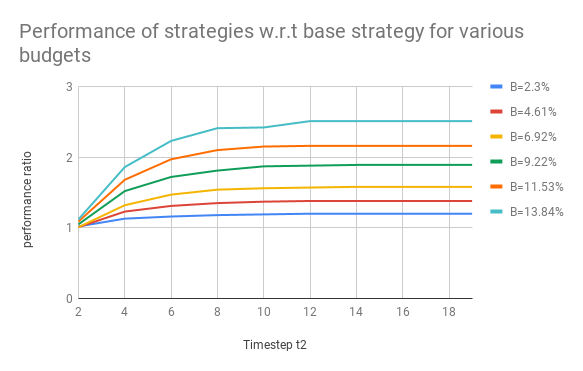
\includegraphics[scale = 0.4]{perf_grqc_eq.png}
    \caption{Performance of various strategies w.r.t base strategy: GrQc, $B_1 = B_2 = \frac{B}{2}$.}
    \label{fig:grqc_performance_eq}
\end{figure}

In Figures \ref{fig:grqc_performance_eq} and \ref{fig:grqc_performance_neq} show the performance of various strategies with respect to the base strategy $t_1 = t_2 = 1$ for the budget distributions (B.i) and (B.ii) respectively. In both these plots, we can notice that for strategies with $t_2$ beyond a certain value (in this case, 6), the performance ratio remains constant. All the strategies have better performance ratio for budget distribution (B.ii) in comparison to (B.i). The epi-curves in Figures [\ref{fig:epicurveGrQc}, \ref{fig:epicurveHepTh}] show that the peak number of infections in each dendograms appears, the peak of the epidemic curve (epi-curve), appears before time step $t = 6$. This provides information on the plateauing of the curves in Figures \ref{fig:grqc_performance_eq} and \ref{fig:grqc_performance_neq}.


\begin{figure}[!h]
    \centering
    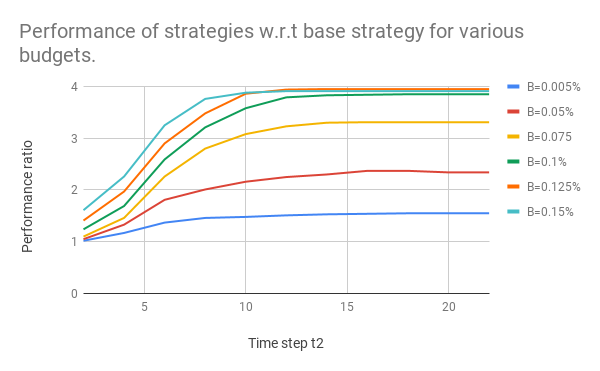
\includegraphics[scale = 0.5]{figures/perf_hepth_eq.png}
    \caption{Performance of various strategies w.r.t base strategy: Hepth, $B_1 = B_2 = \frac{B}{2}$.}
    \label{fig:hepth_performance_eq}
\end{figure}

\begin{figure}[!h]
    \centering
    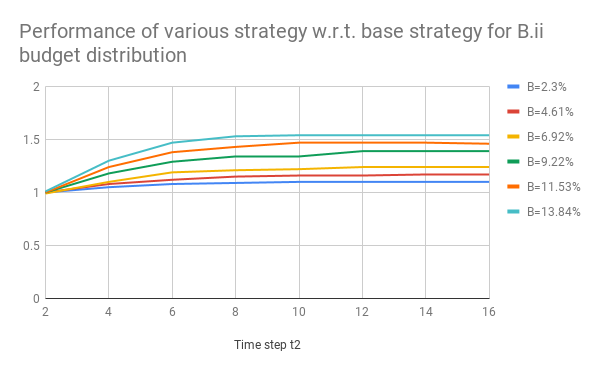
\includegraphics[scale = 0.5]{figures/perf_grqc_neq.png}
    \caption{Performance of various strategies w.r.t base strategy: GrQc, $B_1 = \frac{3B}{4}$ and $B_2 = \frac{B}{4}$.}
    \label{fig:grqc_performance_neq}
\end{figure}


\begin{figure}[!h]
    \centering
    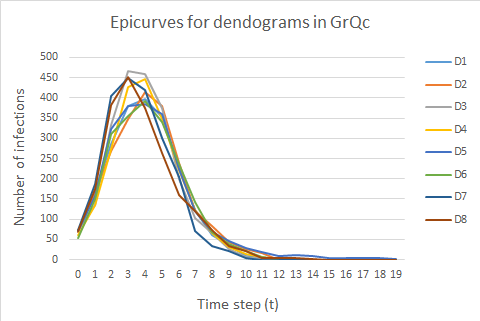
\includegraphics[scale = 0.6]{epicurve-grqc.png}
    \caption{GrQc: Epi-curves for dendograms for $p=0.3$. The x-axis corresponds to the time step $t$ and the y-axis corresponds to the number of infections.}
    \label{fig:epicurveGrQc}
\end{figure}

\begin{figure}[!h]
    \centering
    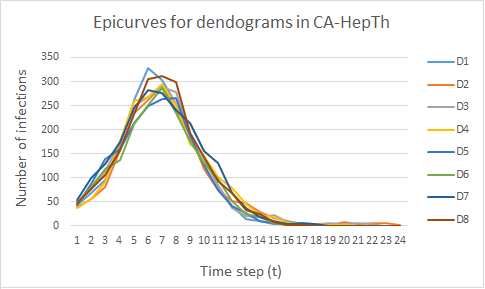
\includegraphics[scale = 0.6]{epicurve-hepth.png}
    \caption{HepTh: Epi-curves for dendograms for $p =0.15$. The x-axis corresponds to the time step $t$ and the y-axis corresponds to the number of infections.}
    \label{fig:epicurveHepTh}
\end{figure}

%\bibliographystyle{named}
%\bibliography{references.bib}


\newpage
\subsection{Adaptive Interventions:}

\textbf{Experimental Setup}

1. In the adaptive case, we assume that the information about the infected nodes is available with certain delay $\tau$. 

2. \textbf{Intervention method 1: (IM1)} The interventions in this method are performed at a time step $T = t$ at which time the information of nodes infected till time $T = t-\tau$ is available. 

3. \textbf{Intervention method 2: (IM2)} The interventions in this method are performed in a two-stage manner. 
The first intervention is performed at $T = 0$ and the second intervention is performed at $T = t$, where information till time $T = t- \tau $ is available.\\ ( need to add the plots after further experimentation.)

\noindent
\textbf{Questions}

1. What is the impact of varying $\tau$ on the quality of interventions in IM1 strategy? \\

Figures \ref{fig:T12tau}, \ref{fig:T7tau} show that the average \% infected increases with the increase in $\tau$ value, for a fixed $T = t$ and budget $B$.
\begin{figure}[!h]
    \centering
    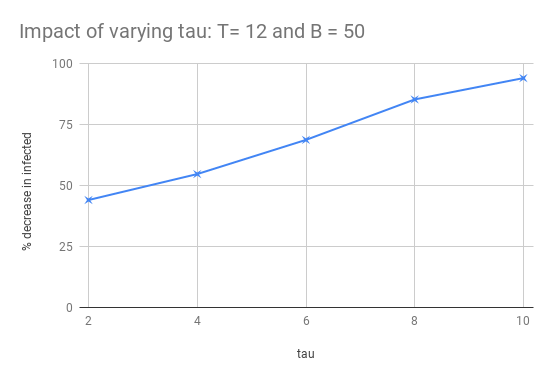
\includegraphics[scale = 0.4]{t12b50tau.png}
    \caption{Impact of varying $\tau$ for T = 12 and B = 50: CA-GrQc}
    \label{fig:T12tau}
\end{figure}

\begin{figure}[!h]
    \centering
    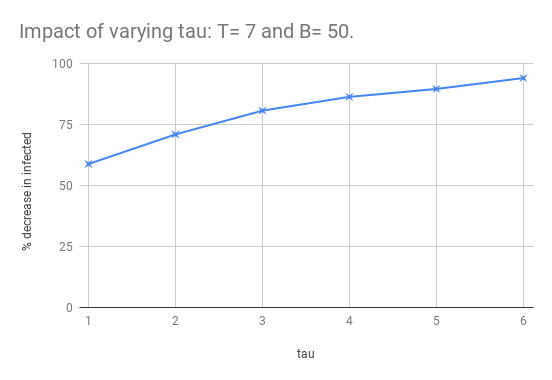
\includegraphics[scale = 0.4]{t7b50tau.png}
    \caption{Impact of varying $\tau$ for T = 7 and B = 50: CA-GrQc}
    \label{fig:T7tau}
\end{figure}

\pagebreak
2. What is benefit of having information if the interventions are performed as per strategy IM1 at time $T = t$? How does the budget $B$ impact this benefit? \\

Figures \ref{fig:benefitGrQc} and \ref{fig:benefit1GrQc} show that the intervention strategies with information at a given time step $T = t$ perform better than without information even with a smaller budget. \\

The impact of budget on this benefit of having information is shown in Figure \ref{fig:budgetvariation}. As the budget increases, the performance gap between strategies with and without information widens.

\begin{figure}[!h]
    \centering
    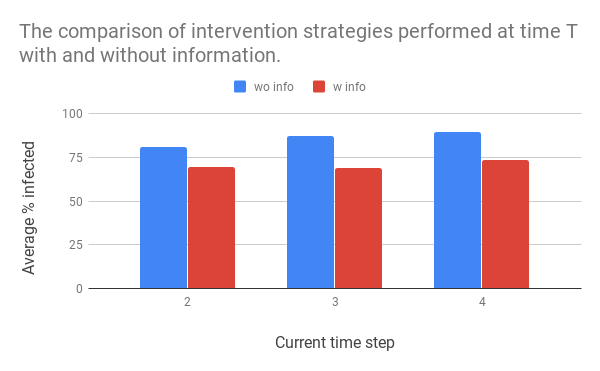
\includegraphics[scale = 0.42]{infobenefit.png}
    \caption{Benefit of having information about previous infections: CA-GrQc. $\tau =2$ and $B = 50$.}
    \label{fig:benefitGrQc}
\end{figure}

\begin{figure}[!h]
    \centering
    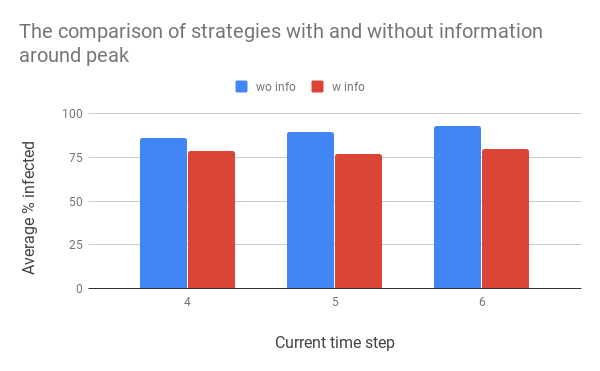
\includegraphics[scale = 0.42]{infobenefit1.png}
    \caption{Benefit of having information about previous infections: CA-GrQc. Current time step around peak. $\tau =2$ and $B = 50$.}
    \label{fig:benefit1GrQc}
\end{figure}

\begin{figure}[!h]
    \centering
    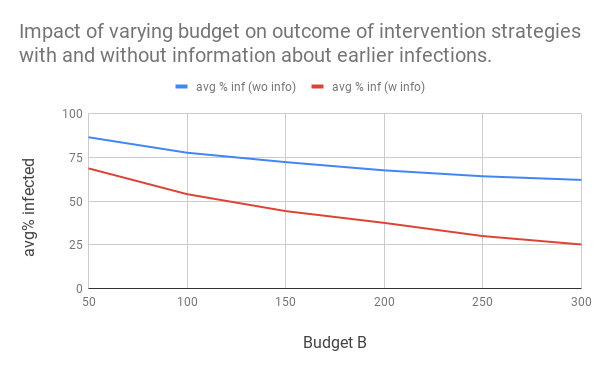
\includegraphics[scale = 0.42]{budgetvariation.png}
    \caption{Impact of varying budget on outcome of intervention stragies with and without information: CA-GrQc, $\tau = 2$, $T = 4$.}
    \label{fig:budgetvariation}
\end{figure}

\pagebreak
3. How does the probability of infections $p$ impact the strategy IM1? \\

Figure \ref{fig:pvalue} shows the impact of probability of infections $p$ on the performance of strategies. As the probability $p$ increases the performance decreases across strategies with information. The strategies with out information having medium and high rates of infections fare poorly in comparison to their counterparts (i.e. with information).

\begin{figure}[!h]
    \centering
    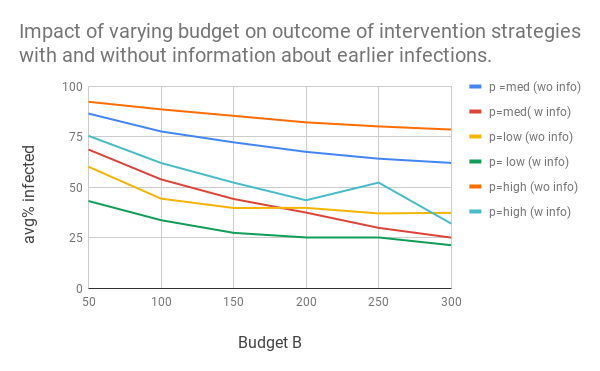
\includegraphics[scale = 0.45]{varyingpvalues.png}
    \caption{Impact of varying probability of infection transmission $p \in \{low =0.1, med = 0.3, high = 0.5\}$: CA-GrQc, $\tau = 2$, $T = 4$.}
    \label{fig:pvalue}
\end{figure}

\pagebreak
4. How does the strategy IM1 for a $T = t$ compare to performing interventions at the start? How long can one delay intervention to get information?

\begin{figure}[!h]
    \centering
    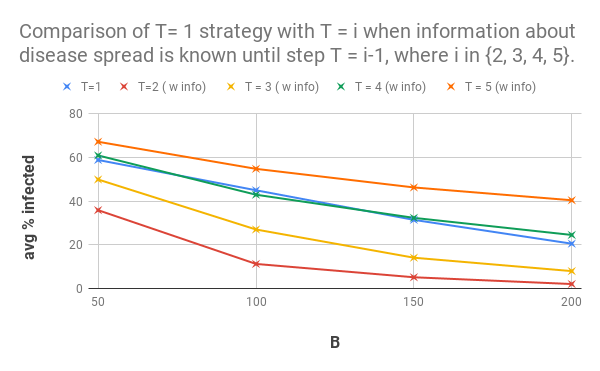
\includegraphics[scale = 0.42]{tau1.png}
    \caption{Comparison of the strategy T = 1 with T = i when the information about disease spread is known till T= i-1, i.e. $\tau = 1$, where $T \in \{2, 3, 4, 5\}$}
    \label{fig:tau1}
\end{figure}

\begin{figure}[!h]
    \centering
    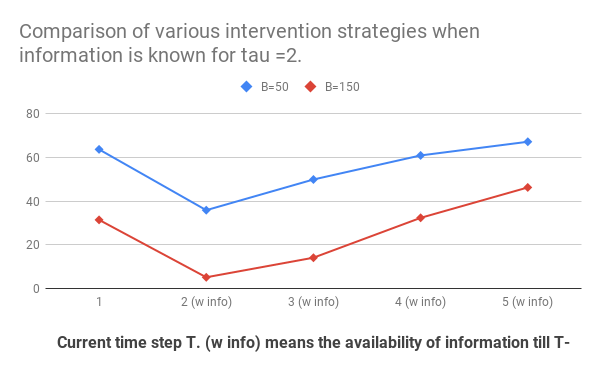
\includegraphics[scale = 0.42]{tau2.png}
    \caption{Comparison of the strategy T = 1 with T = i when the information about disease spread is known till T=i-2, i.e. $\tau = 2$, where $T \in \{2, 3, 4, 5\}$}
    \label{fig:tau2}
\end{figure}

\begin{figure}[!h]
    \centering
    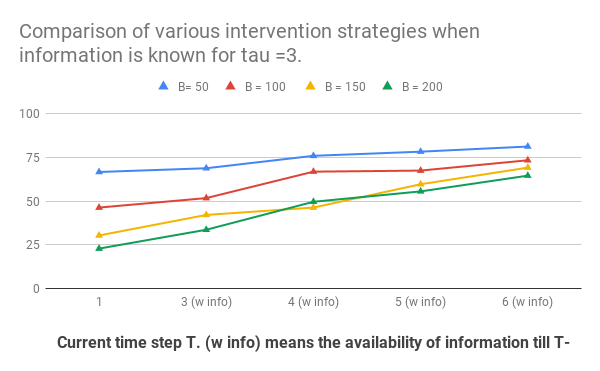
\includegraphics[scale = 0.42]{tau3.png}
    \caption{Comparison of the strategy T = 1 with T = i when the information about disease spread is known till T=i-3, i.e. $\tau = 3$, where $T \in \{3, 4, 5, 6\}$}
    \label{fig:tau3}
\end{figure}

\begin{figure}[!h]
    \centering
    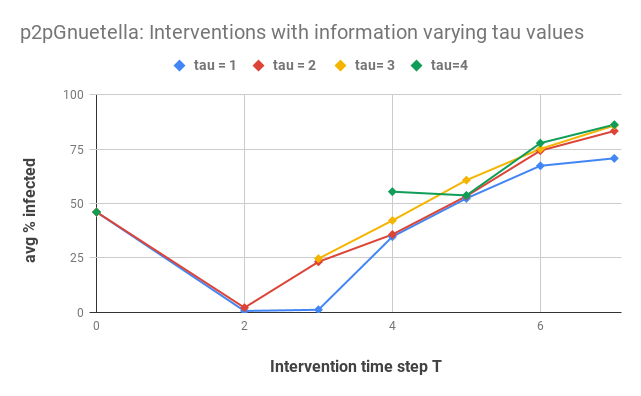
\includegraphics[scale = 0.42]{p2ptau1to4.png}
    \caption{Comparison of the intervention strategies with information while varying $\tau \in [1,4]$. X-axis corresponds to the time step at which intervention is performed. Y-axis corresponds to the \% average infected.}
    \label{fig:p2p2tau1to4}
\end{figure}

\begin{figure}[!h]
    \centering
    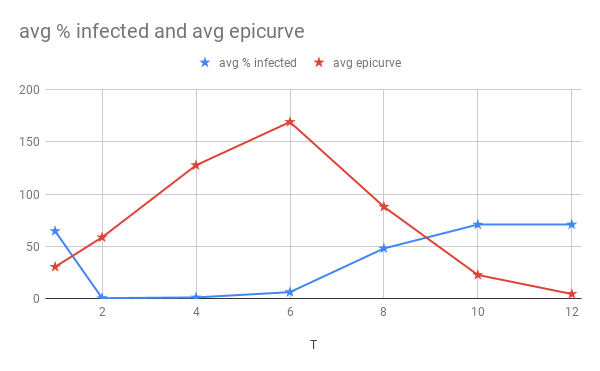
\includegraphics[scale = 0.42]{sw1.png}
    \caption{Small world network with $n = 1000, k = 10, p = 0.1$. Intervention with information. $\tau = 2$ and $B = 100$. The red curve corresponds to the average epi-curve.}
    \label{fig:sw1}
\end{figure}

\


\begin{figure}[!h]
    \centering
    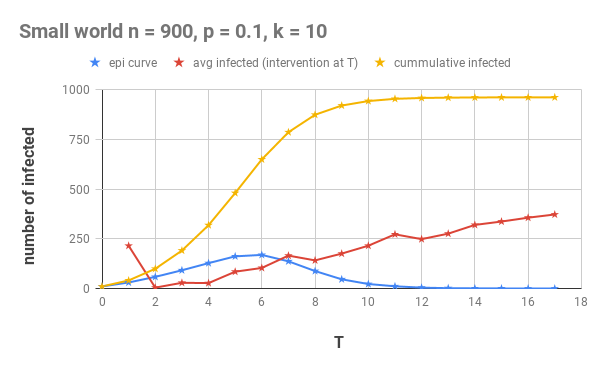
\includegraphics[scale = 0.42]{sw2.png}
    \caption{Small world network (Kleinberg) with $n = 900,p =1, q =1, r =2, dim = 2$. Average epicurve vs. Cummulative Infections vs. average infected after intervention at $T$.$B = 50, \tau = 2$.}
    \label{fig:sw2}
\end{figure}

\section{Experiments on Small World Networks}
We generate a small world network based on Kleinberg's model [cite] with 2500 nodes on a grid. The average epicurve is computed based on the average obtained over 50 simulations of the epidemic spread with the probability of infection $p = 0.3$. In Figures [\ref{fig:sw2500tau1}, \ref{fig:sw2500tau3}], the average infected after intervening at time step $T$ is presented along with the average epicurve and the average cumulative infected. The average epicurve is the average number of infected at each time step over 50 simulations. The average cumulative (refered to as cumulative) infected is the average cumulative infected at each time step over all the simulations. The average infected after intervention at $T$ is the average number of infected over all the simulations after some nodes are removed from network after intervention. 

\textbf{Observations:}
1. The peak is around $T = 10$.
2. The cumulative infected plateaus after $T = 20$. This implies that only few people are newly infected after 20 time steps.
3. In both Figures [\ref{fig:sw2500tau1}, \ref{fig:sw2500tau3}], it can be seen that the benefit of having information before interventions in comparison to doing all the interventions at $T=1$ starts to decrease just after the peak. [experiments running for $\tau = 2$.] 
\begin{figure}[!ht]
    \centering
    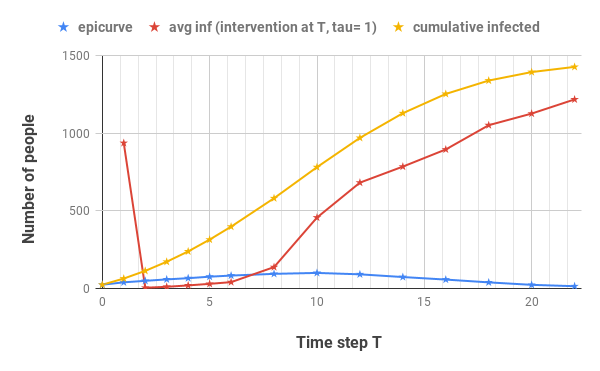
\includegraphics[scale = 0.42]{sw2500tau1.png}
    \caption{Small world network (Kleinberg) with $n = 50,p =1, q =1, r =2, dim = 2$ as parameters. Average epicurve vs. Cummulative Infections vs. average infected after intervention at $T$.$B = 100, \tau = 1$.}
    \label{fig:sw2500tau1}
\end{figure}

\begin{figure}[!ht]
    \centering
    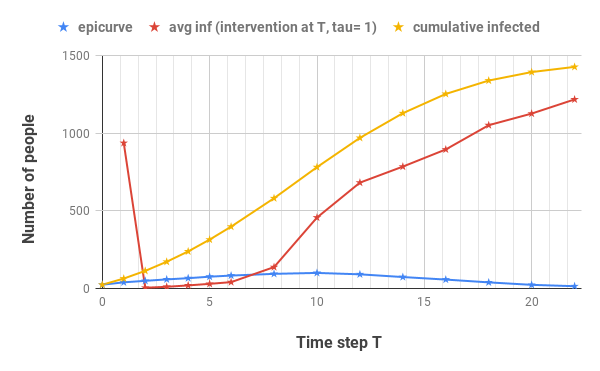
\includegraphics[scale = 0.42]{sw2500tau1.png}
    \caption{Small world network (Kleinberg) with $n = 50,p =1, q =1, r =2, dim = 2$ as parameters. Average epicurve vs. Cummulative Infections vs. average infected after intervention at $T$.$B = 100, \tau = 3$.}
    \label{fig:sw2500tau3}
\end{figure}
